\documentclass[11pt,spanish]{article} % Idioma
\usepackage{babel}
\usepackage[T1]{fontenc}
\usepackage{textcomp, verbatim} % \begin{comment}
\usepackage[utf8]{inputenc} % Permite acentos

\usepackage{wrapfig} % Imagenes %\graphicspath{ {./imagenes/} }
\usepackage[left=2.75cm,top=2.5cm,right=2cm,bottom=2.5cm]{geometry} % Márgenes
\usepackage{amssymb, amsmath, amscd, amsfonts, amsthm, mathrsfs } % Símbolos matemáticos
\usepackage{cancel} % Cancelar expresiones
\usepackage{multirow, multicol, tabularx, booktabs, longtable} % Tablas
\usepackage{fancyhdr, fncychap} % Encabezados
\usepackage{algpseudocode, algorithmicx, algorithm} % Pseudo-código
\usepackage{bbding} % Símbolos
\usepackage{enumitem} % Enumerados a), b), c)... usando \begin{enumerate}[label=\alph*)]
\usepackage{graphicx, xcolor, color, pstricks} % Gráficos --TikZ--
% http://www.texample.net/tikz/examples/
\usepackage[hidelinks]{hyperref}  % Enlaces
\usepackage{verbatim} % Comentarios largos \begin{comment}
\usepackage{rotating} % \begin{rotate}{30}
\usepackage[all]{xy} % Diagramas
\usepackage{xparse} % Entornos
\usepackage{listings}

\definecolor{codegreen}{rgb}{0,0.6,0}
\definecolor{codegray}{rgb}{0.5,0.5,0.5}
\definecolor{codepurple}{rgb}{0.58,0,0.82}
\definecolor{backcolour}{rgb}{0.95,0.95,0.92}

\lstdefinestyle{mystyle}{
	backgroundcolor=\color{backcolour},
	commentstyle=\color{codegreen},
	keywordstyle=\color{magenta},
	numberstyle=\tiny\color{codegray},
	stringstyle=\color{codepurple},
	basicstyle=\footnotesize,
	breakatwhitespace=false,
	breaklines=true,
	captionpos=b,
	keepspaces=true,
	numbers=left,
	numbersep=5pt,
	showspaces=false,
	showstringspaces=false,
	showtabs=false,
	tabsize=2
}
\lstset{style=mystyle}


% Comandos
\newcommand{\docdate}{}
\newcommand{\subject}{}
\newcommand{\docauthor}{Rubén Morales Pérez}
\newcommand{\docemail}{srmorales@correo.ugr.es}

\newcommand{\N}{\mathbb{N}}
\newcommand{\Q}{\mathbb{Q}}
\newcommand{\C}{\mathbb{C}}
\newcommand{\R}{\mathbb{R}}
\newcommand{\Z}{\mathbb{Z}}




\usepackage[final]{pdfpages}


\linespread{1.1}                  % Espacio entre líneas.
\setlength\parindent{0pt}         % Indentación para párrafo.

\title{INGENIERÍA DE REQUISITOS \\
	Análisis y especificación de requisitos}
\author{Alicia Rodríguez Gómez \\
	Francisco Javier Morales Piqueras \\
	Rubén Morales Pérez \\
	Samia Mikou}
\date{\today}

% % % % % % % % % % % % % % % % % % % % % % % % % % % % % % % % %
%					 Inicio del documento
% % % % % % % % % % % % % % % % % % % % % % % % % % % % % % % % %
\begin{document}

\maketitle
\tableofcontents % Generando el indice
\setlength\parindent{0pt} % Quitamos la sangría
\newpage 

\vspace{5cm}
\section{Introducción}
En este documento se elabora el modelo conceptual o modelo de dominio del problema usando un diagrama de clases de UML, también se desarrollan los diagramas de secuencia del sistema (DSS)



\section{Diagrama de secuencia administración de usuarios}
\begin{figure}[H]
	\centering
	\label{ModeloConceptual}
	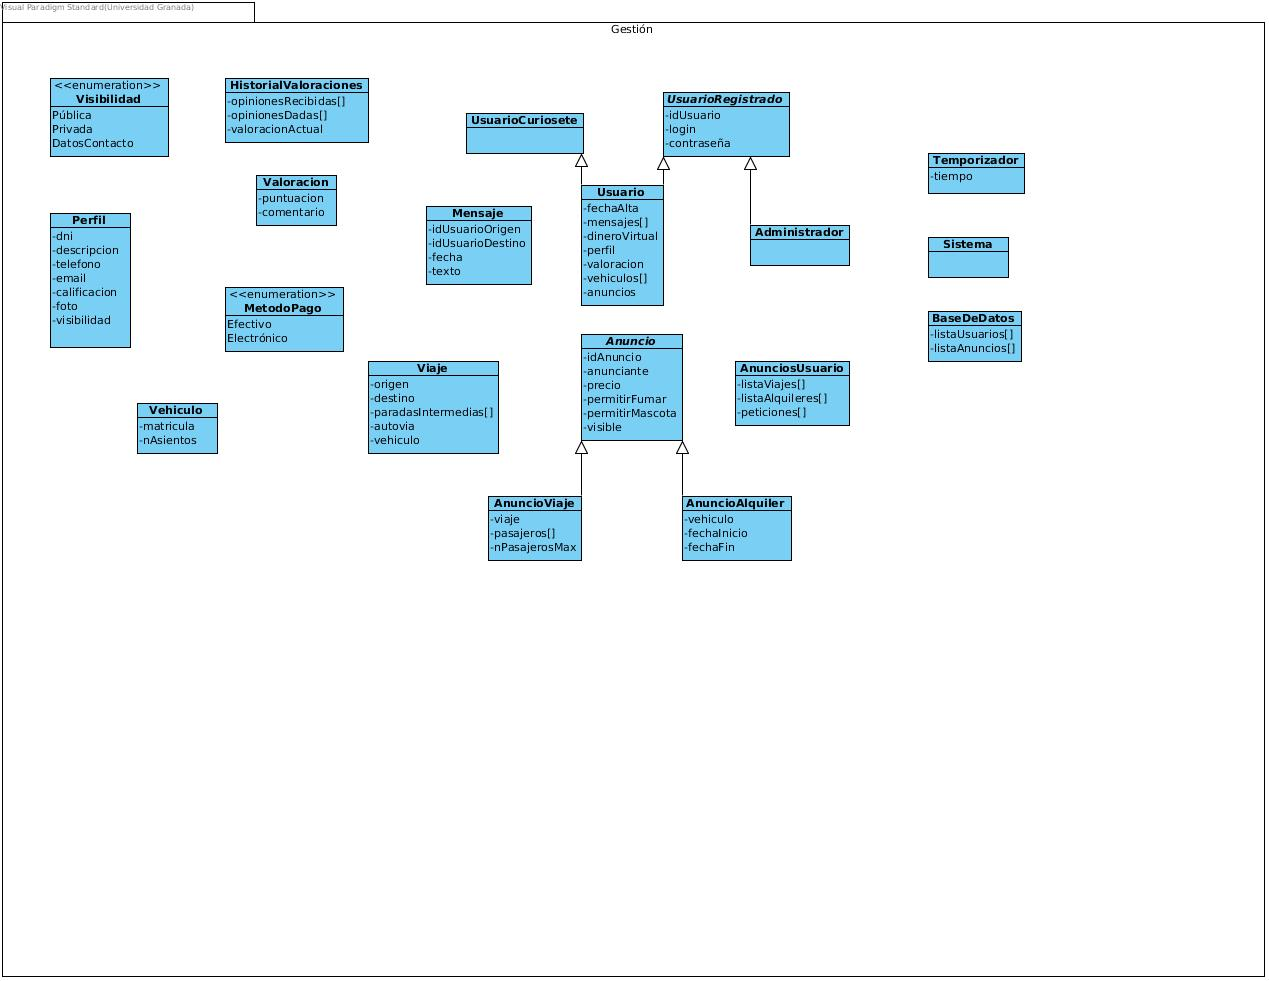
\includegraphics[scale=0.4]{./ModeloConceptual.jpg}
	\caption{Modelo conceptual del problema}
\end{figure}

\section{Diagrama de secuencia administración de usuarios}
\begin{figure}[H]
	\centering
	\label{AdministracionUsuarios}
	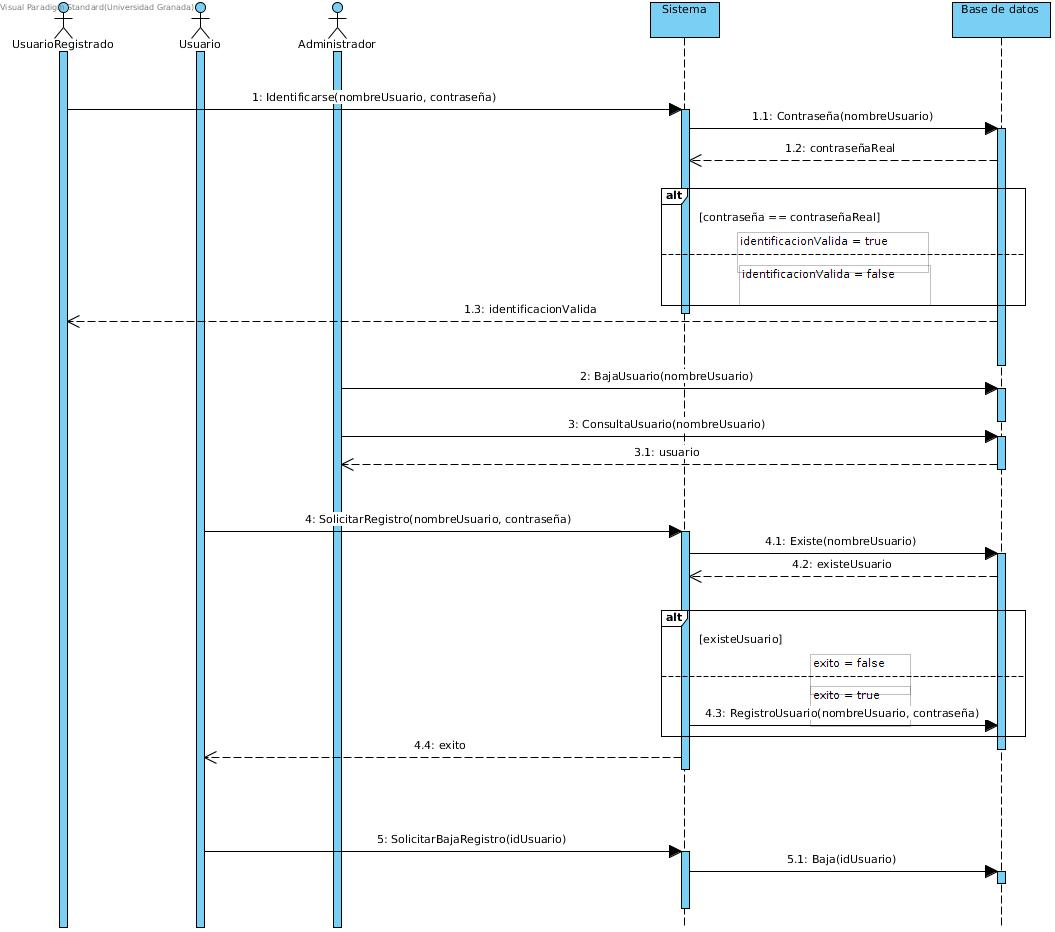
\includegraphics[scale=0.4]{././DiagramasSecuencia/AdministracionUsuarios.jpg}
	\caption{Diagrama de secuencia administración de usuarios}
\end{figure}

\section{Diagrama de secuencia gestión de perfil}
\begin{figure}[H]
	\centering
	\label{GestionPerfil}
	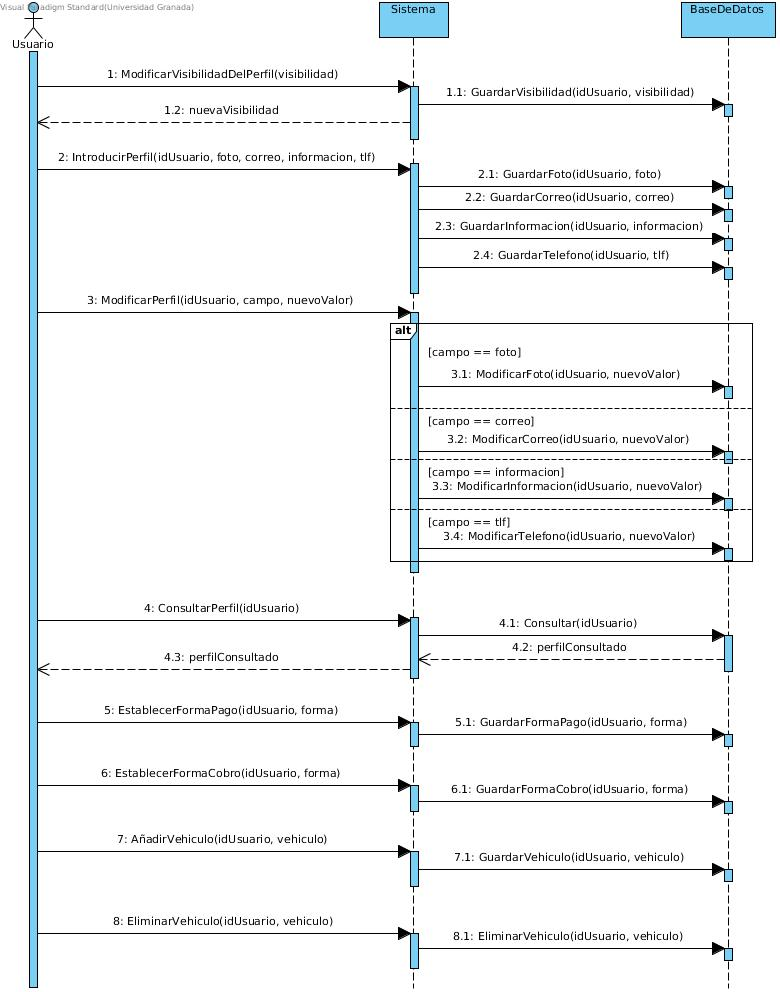
\includegraphics[scale=0.5]{././DiagramasSecuencia/GestionPerfil.jpg}
	\caption{Diagrama de secuencia gestión de perfil}
\end{figure}

\section{Diagrama de secuencia gestión de viajes}
\begin{figure}[H]
	\centering
	\label{GestionViaje}
	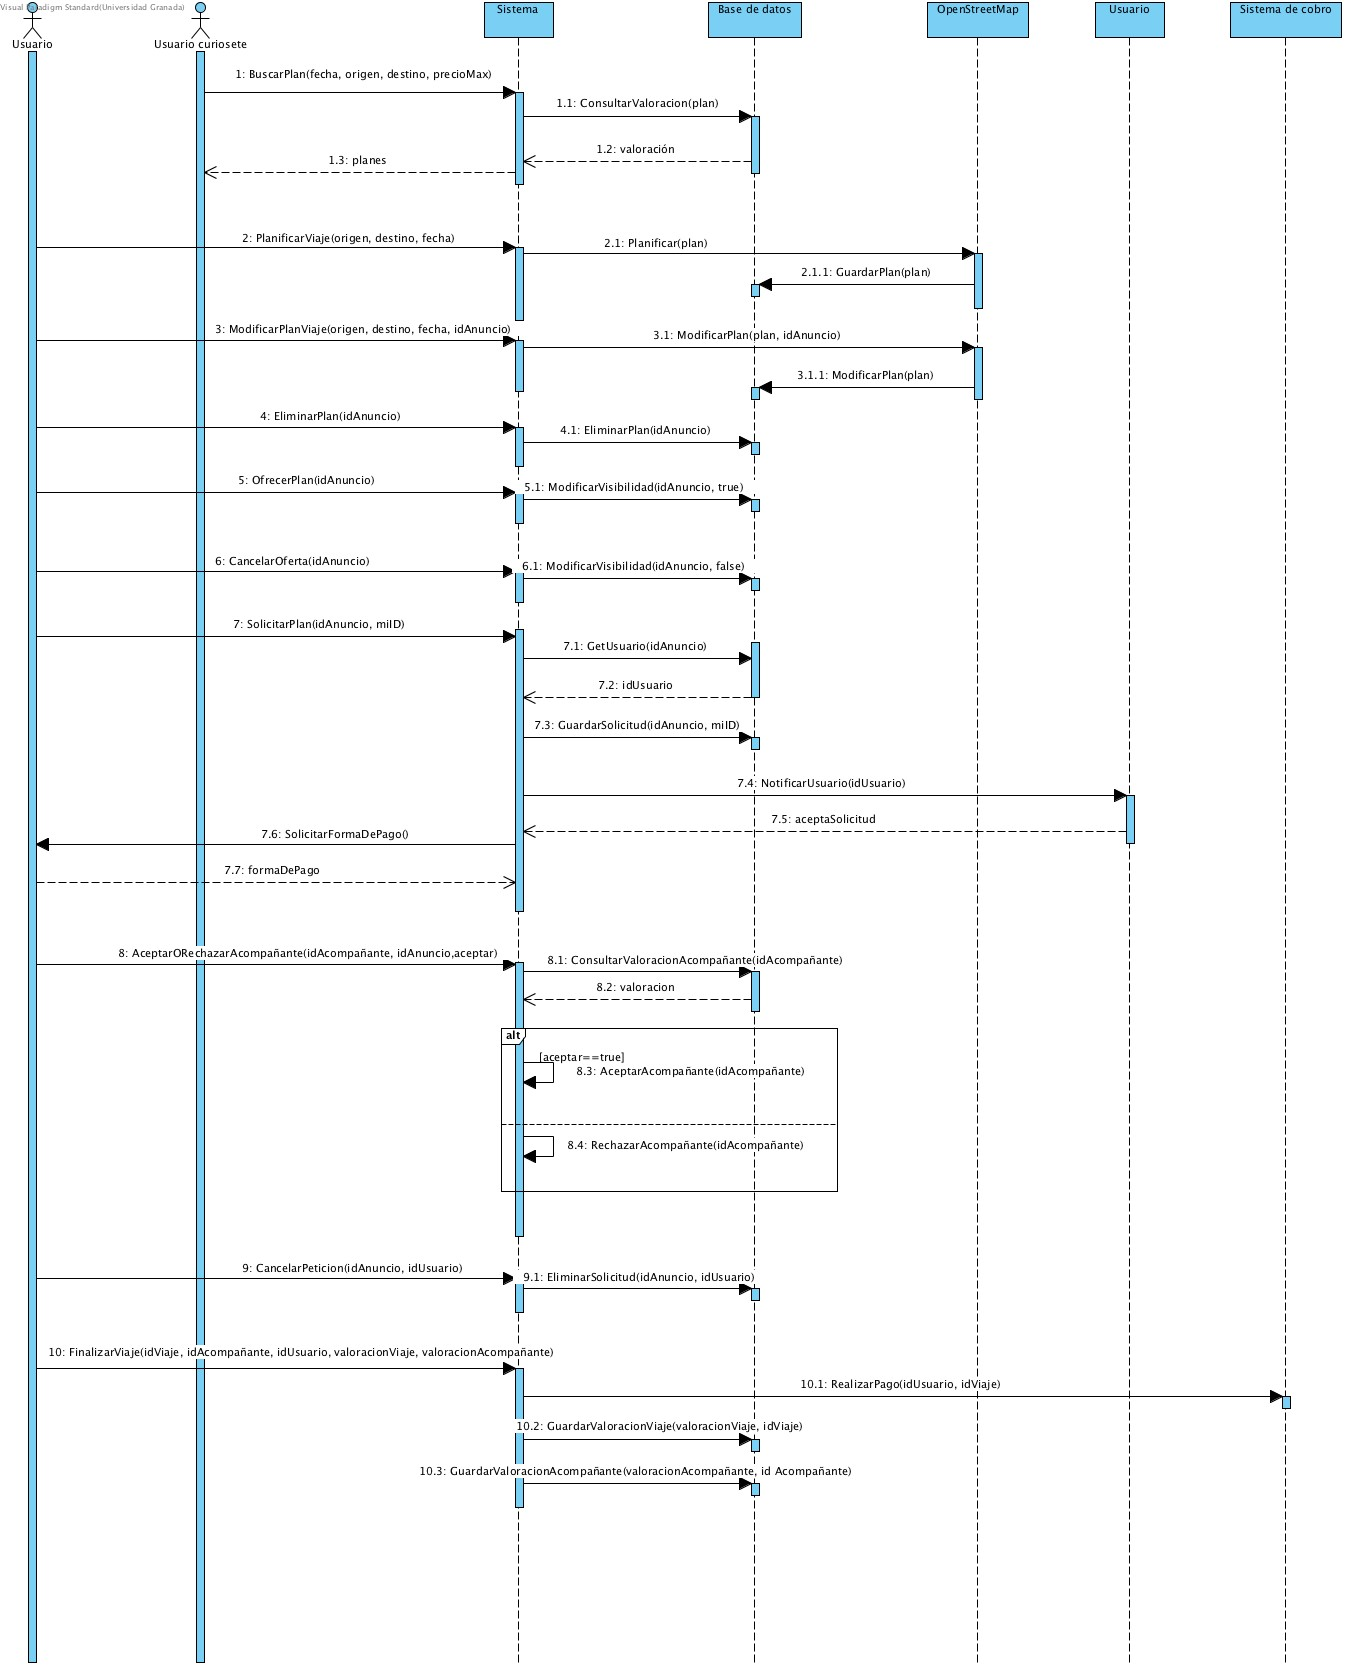
\includegraphics[scale=0.352]{././DiagramasSecuencia/GestionViajes.jpg}
	\caption{Diagrama de secuencia gestión de viajes}
\end{figure}

\section{Diagrama de secuencia gestión de alquileres}
\begin{figure}[H]
	\centering
	\label{GestionAlquileres}
	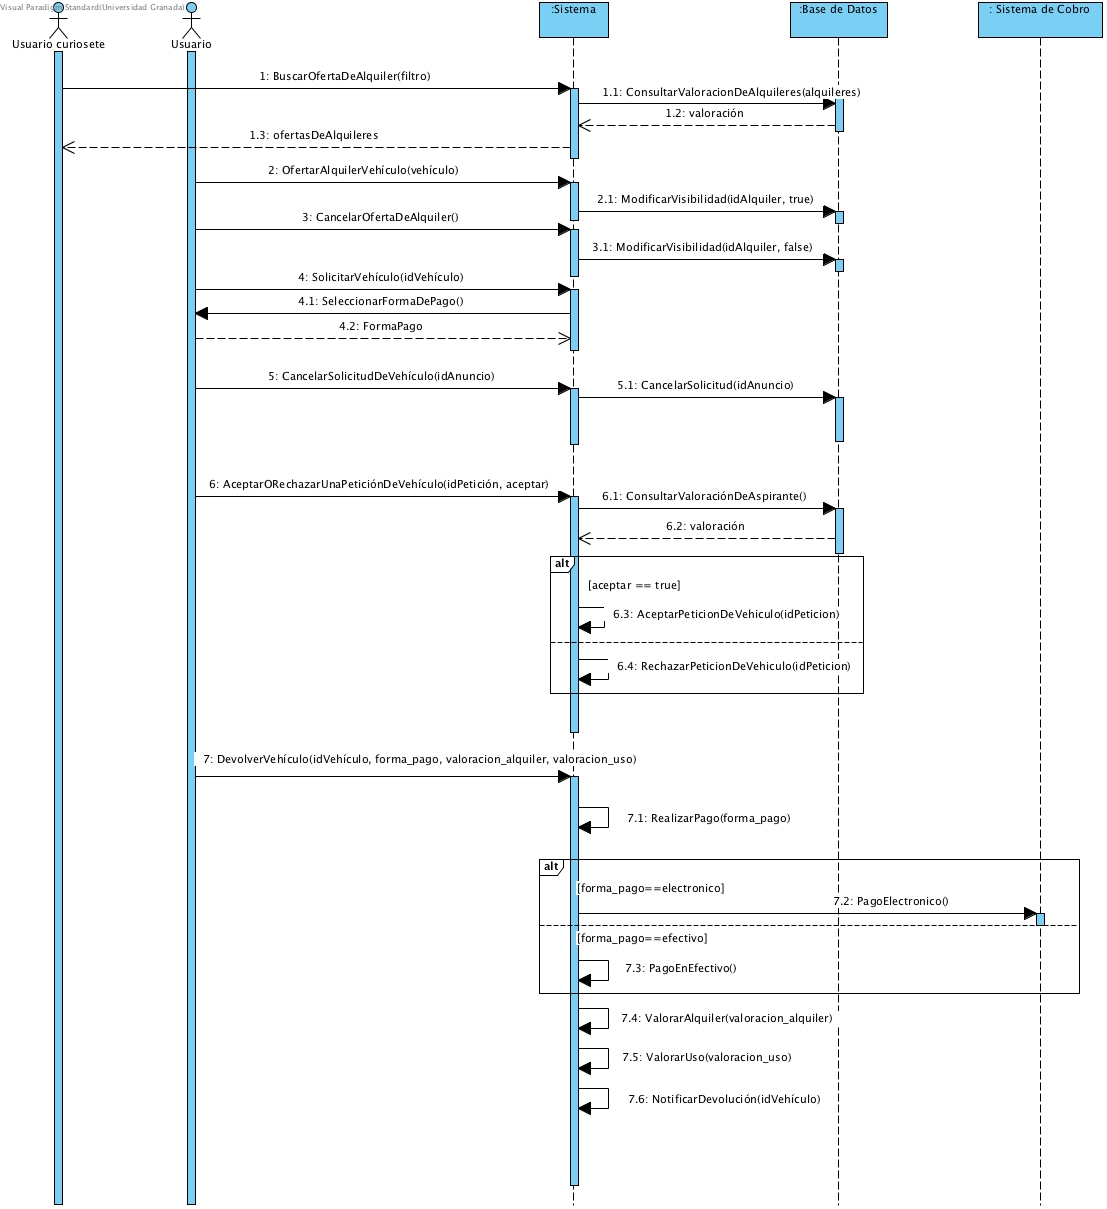
\includegraphics[scale=0.4]{././DiagramasSecuencia/GestionAlquiler.jpg}
	\caption{Diagrama de secuencia gestión de alquileres}
\end{figure}

\subsection{Diagrama de secuencia temporizador}
\begin{figure}[H]
	\centering
	\label{GestionTemporizador}
	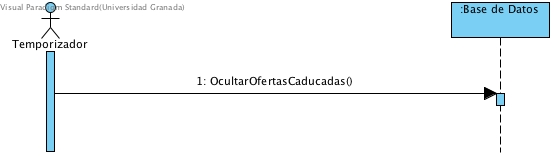
\includegraphics[scale=0.5]{././DiagramasSecuencia/Temporizador.jpg}
	\caption{Diagrama de secuencia gestión del temporizador}
\end{figure}

\section{Diagrama de secuencia gestión de comunicaciones e incidencias}
\begin{figure}[H]
	\centering
	\label{GestionComunicacionesIncidencias}
	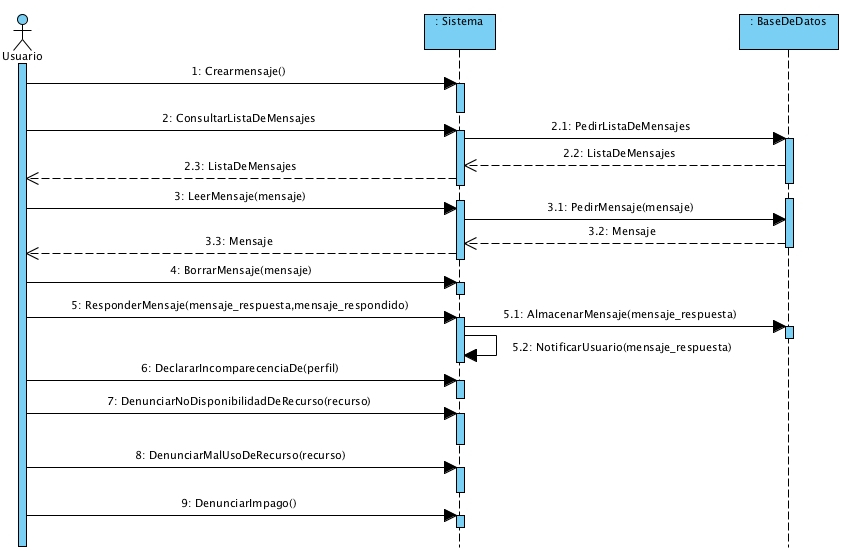
\includegraphics[scale=0.5]{././DiagramasSecuencia/GestiondeComunicacion.jpg}
	\caption{Diagrama de secuencia gestión de las comunicaciones e incidencias}
\end{figure}


\end{document}
